\documentclass[12pt]{article}
\usepackage[a4paper, margin=.30in]{geometry}
\usepackage{graphicx ,
            wrapfig,
            xcolor, 
            enumerate,
            amsmath,fontenc, mhchem
            }

\newcommand\headerMe[2]{\noindent{}#1\hfill#2}
\renewcommand{\thesection}{\Roman{section}}

\author{Zakaria HAOUZAN}
\date{\today}

\begin{document}
% headers --------------
\headerMe{Matière : Physique-Chimie}{Professeur : Zakaria HAOUZAN}\\
\headerMe{Unité : Transformations lentes et rapides\\ d'un système chimique }{Établissement : Lycée SKHOR qualifiant}\\
\headerMe{Niveau : 2BAC-SM-X}{Heure : 11H}\\

% ------Content ________
\begin{center}

    \Large{Leçon $N^{\circ} 2 $: \color{red} Transformations lentes et rapides }
\end{center}

%\begin{wrapfigure}[10]{r}{0.5\textwidth}
%    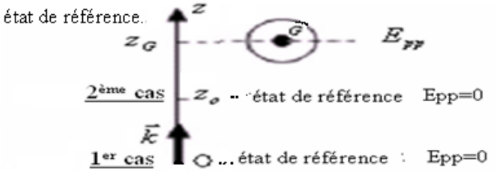
\includegraphics[width=0.5\textwidth]{./img/img00.png}
%\end{wrapfigure}


%\begin{center}
   %\begin{tabular}{|c|c|c|}
      %\hline
      %Indicateur coloré & Couleur de l’espèce acide & Couleur de l’espèce base\\\hline
      %BBT               & Jaune                     & Bleue\\\hline
      %Hélianthine       &Rose                       & Jaune\\\hline
      %Phénolphtaléine   & inclore                   & rose \\\hline
   %\end{tabular}
%\end{center}
\section{Rappels sur les couples Ox/Red : }
\begin{itemize}
	\item L'oxydation est une perte d'un ou plusieurs électrons. La réduction est un gain d'un ou plusieurs électrons.
	\item  Un oxydant est une espèce chimique capable de capter un ou plusieurs électrons au cours d'une transformation chimique.
	\item Un réducteur est une espèce chimique capable de céder un ou plusieurs électrons au cours d'une transformation chimique.
	\item Chaque couple Ox/Red est caractérisé par sa demi-équation d'oxydoréduction: \ce{ox + ne^- -> red}
	\item Exemple : 

		\ce{$\underset{\text{réducteur}}{\ce{Fe}}$ ->[\text{oxydation}]$\underset{\text{oxydant}}{\ce{Fe^{3+}}}$  + 3e^-} ; 
		\hspace{5cm}	\ce{$\underset{\text{oxydant}}{\ce{Fe^{3+}}}$  + 3e^-  ->[\text{réduction}]  $\underset{\text{réducteur}}{\ce{Fe}}$   } ;
Au cours d'une oxydation le réducteur s'oxyde et au cours d'une réduction l'oxydant se réduit.
Les deux transformations sont possibles donc, on associe au couple $Fe^{3+}/Fe$ la demi-équation d'oxydo-réduction :

\item Une réaction d'oxydoréduction est caractérisée par un transfert d'électrons entre l'oxydant d'un couple $ox_1/red_1$ et le
réducteur d'un autre couple $ox_2/red_2$.
\item Au cours de cette réaction, l'oxydant ox1 capte des électrons : on dit qu'il subit une réduction, le réducteur red2 cède des
électrons : on dit qu'il subit une oxydation.
\item L'équation bilan de la réaction s'obtient en " additionnant " les deux demi-équations de la manière suivante: \ce{n_2OX_1 + n_1RED_2 -> n_2RED_1 + n_1OX_2}

\end{itemize}
\section*{exercices d'application 1  : }
\begin{enumerate}
	\item Écrire les demi-équations d'oxydo-réduction pour chacun des couples suivants: $Al^{3+}/Al$ ; $Cl_2/Cl^-$ ; $MnO_4^-/Mn^{2+}$ ; $Fe^{3+}/Fe^{2+}$
	\item Écrire l'équation d'oxydo-réduction entre les ions ferreux $Fe^{2+}$ et les ions permanganates $MnO_4^-$ en milieu acide sachant que  
\end{enumerate}

\begin{wrapfigure}[2]{r}{0.2\textwidth}
	\vspace{-1.95cm}
	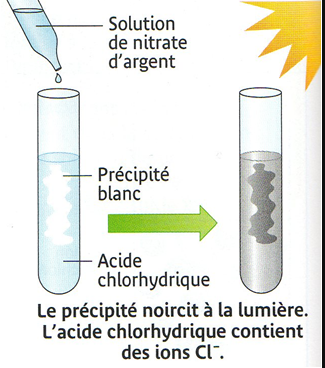
\includegraphics[width=0.2\textwidth]{./img/TRLprecipitationChlorure.png}
\end{wrapfigure}


\section{Transformations lentes et transformations rapides : }
\subsection{Transformations rapides :  }
\subsubsection{ Définition: }
Une transformation rapide est une transformation qui se fait en une courte durée de telle façon qu'on ne peut pas suivre son
évolution en fonction du temps avec l'œil ou avec les appareils de mesure.

\subsubsection{Exemples:}

\section*{Précipitation du chlorure d'argent.}
On verse dans un tube à essaies une solution de nitrate d'argent $(Ag^+ + NO_3^-)$ ,puis on lui ajoute une solution d'acide chlorhydrique $(H_3O^+  + Cl^-)$

On constate la formation d'un précipité blanc de chlorure d'argent AgCl (qui noirci à la lumière) selon une réaction rapide dont l'équation s'écrit:

\ce{Ag^+_{(aq)} + Cl^-_{(aq)} -> AgCl_{(s)}}

\section*{Précipitation de l'hydroxyde de fer III.}
On verse dans un tube à essaies une solution de chlorure de fer III $(Cl^- +Fe^{3+} )$ puis on lui ajOute une solution d'hydroxyde de sodium $(Na^+ + OH^-)$
solution d'hydroxyde de sodium

On constate la formation d'un précipité de couleur rouille d'hydroxyde de fer III selon une réaction rapide dont l'équation s'écrit: \ce{Fe^{3+}_{(aq)}  + 3HO^-_{(aq)} -> Fe(OH)_3}

\begin{figure}[h!]
	\begin{center}
	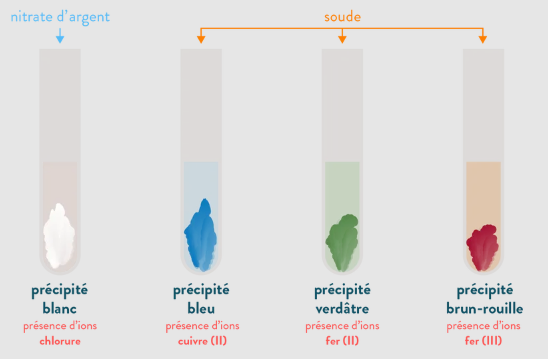
\includegraphics[width=0.5\textwidth]{./img/TRLtestchimique.png}
\end{center}
\vspace{-1cm}
\end{figure}
\begin{wrapfigure}[1]{r}{0.4\textwidth}
	\vspace{-2.45cm}
	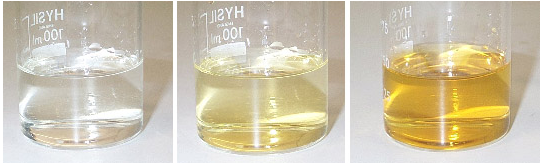
\includegraphics[width=0.4\textwidth]{./img/TRLidurelente.png}
\end{wrapfigure}


\subsection{Transformations lentes :}
\subsubsection{Définition: }
Une transformation lente est une transformation qui se fait dans une certaine durée de telle façon qu'on suivre son évolution en
fonction du temps avec l'œil ou avec les appareils de mesure.

\section*{Exemple: }
Réaction entre les ions iodures $(I^-)$ et l'eau oxygénée $(H_2O_2)$ (peroxyde d'hydrogéne)

\begin{itemize}
	\item On verse dans un tube à essaies une solution d'iodure de potassium $(K^+ + I^-)$ puis on lui ajoute un peu d'eau oxygénée $(H_2O_2)$ acidifiée avec quelques gouttes d'acide sulfurique $H_2SO_4$
	\item Il y'a formation progressive du diiode I2 caractérisé par sa coloration brune .On constate que la couleur du mélange réactionnel
évolue progressivement du jaune au jaune foncé puis prend une coloration brune qui devient de plus en plus foncée en fonction du
temps .
\item Donc la réaction des ions iodures $I^-$ et les molécules $H_2O_2$ est une réaction lente au cours de laquelle les
	ions iodures s'oxydent selon la demi-équation suivante: 

	\ce{2I^- <=> I_2 + 2e^-}
\item Alors que les molécules H2O2 se réduisent selon la demi-équation suivante: 

	\ce{H_2O_2 + 2H^+ + 2e^- <=> 2H_2O}

\item L'équation bilan d'oxydo-réduction: \ce{H_2O_2 + 2I^- + 2H^+ ->[\text{réaction lente}] I_2 + 2H_2O}

\end{itemize}
\section{Les facteurs cinétiques }
\subsection{Définition: }
On appelle facteur cinétique tout paramètre capable d'influer sur la vitesse d'une transformation chimique.

\subsection{Influence des facteur cinétique sur la vitesse de la réaction:}
\subsubsection{Influence de la température: }


\end{document}

